\section{Introduction}






The looming threat of irreversible damage to global ecosystems due to
anthropogenic climate change has motivated many countries to adopt goals to
curb damaging carbon emissions, underscored by the 196 signatories of the 2015
Paris Agreement \cite{noauthor_paris_nodate}. In 2019, the United States made
plans to formally withdraw from the agreement, the only country to do so
\cite{eshraghi_us_2018}. In spite of
this, individual states and institutions have created their own climate goals
conistent with the aims of the Paris Agreement. The \gls{uiuc} is one such
institution. In 2015 \gls{uiuc} published the \gls{icap} with the goal to
become carbon neutral by 2050 or sooner \cite{isee_illinois_2015}. Emissions
projections shown in Figure \ref{fig:icap_emissions} illustrate the needed
policy changes to meet climate goals.

\begin{figure}[h]
  \centering
  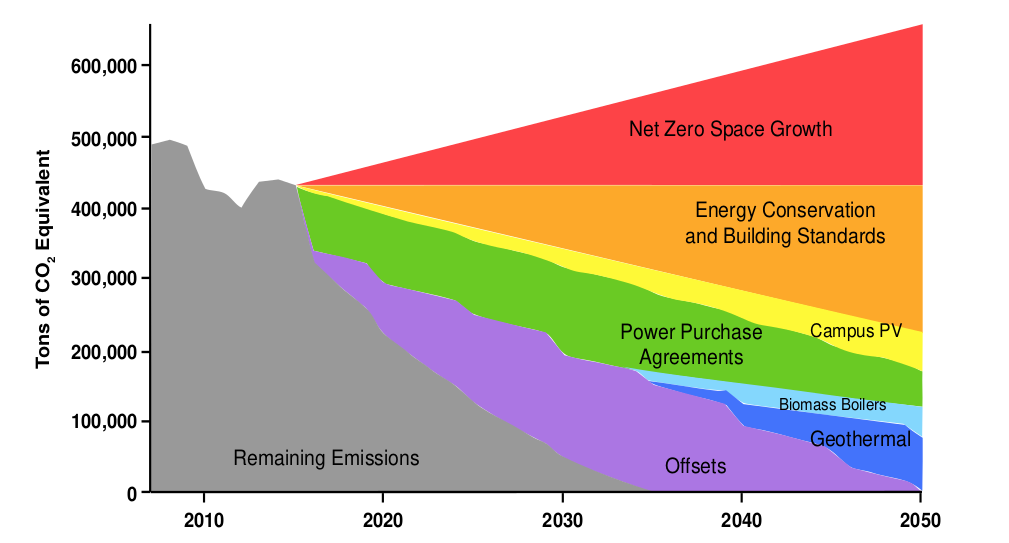
\includegraphics[width=\columnwidth]{icap_uiucemissions.png}
  \caption{The projected carbon emissions with corresponding policy changes.
  ``Offsets" includes shutting down the Blue Waters Supercomputer. Image
  originally published in \gls{icap} 2015 \cite{isee_illinois_2015}.}
  \label{fig:icap_emissions}
\end{figure}

\gls{uiuc} poses an interesting opportunity to explore options for rapid
decarbonization because it: (1) is a mostly self-contained micro-grid (2) has a
diverse mix of energy production and (3) relies on steam for district heating
which challenges decarbonization efforts.


The \gls{icap} goals for \gls{uiuc} include several categories
\cite{isee_illinois_2015}:
\begin{enumerate}
  \item Energy conservation and building standards
  \item Energy generation, purchasing, and distribution
  \item Transportation
  \item Water
  \item Waste and recycling
  \item Agriculture and land use
\end{enumerate}

Energy conservation, generation, and purchasing objectives are of primary
interest because these items account for 88\% of \gls{uiuc}'s emissions, shown
in Figure \ref{fig:uiuc_emissions_breakdown}. \gls{icap} 2015 showed that
\gls{uiuc} made progress towards its emissions goals. Further, in 2016
\gls{uiuc} entered a power purchase agreement with Railsplitter Wind Farm
\cite{breitweiser_wind_2016} and completed Solar Farm 1.0
\cite{white_solar_2017}. Though these investments indicate \gls{uiuc}'s dedication to
emissions goals, they have not been enough to curb emissions as shown in Figure
\ref{fig:uiuc_ghg}.

\begin{figure}[h]
  \centering
  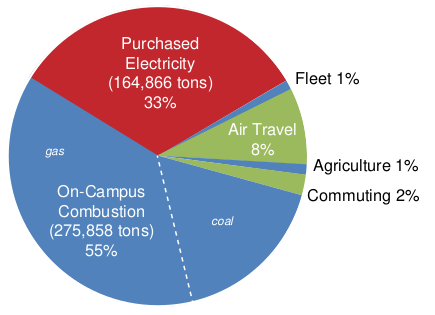
\includegraphics[width=\columnwidth]{uiuc_emissions_breakdown.png}
  \caption{Shows three scopes of university related emissions: on-campus
  (blue), purchased electricity (red), and off-campus (green). Image originally
  published in \gls{icap} 2015 \cite{isee_illinois_2015}.}
  \label{fig:uiuc_emissions_breakdown}
\end{figure}

\begin{figure}[h]
  \centering
  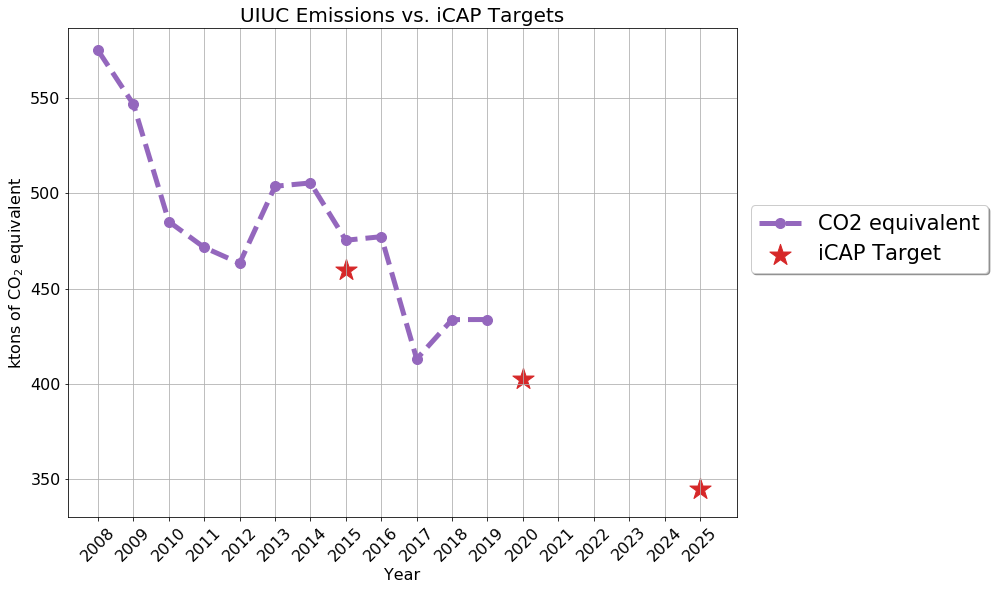
\includegraphics[width=\columnwidth]{uiuc_ghgtargets.png}
  \caption{\gls{uiuc}'s actual net emissions compared with \gls{icap}'s
  stated goals. Data taken from the iCAP Sustainability Portal
  \cite{noauthor_metric_nodate}.}
  \label{fig:uiuc_ghg}
\end{figure}

The struggle to meet these climate goals demonstrates the challenge decision
makers face in balancing stakeholder interests, cost, and sustainability goals.
The 2015 Facilities and Services Master Plan, used to define the needs of the
\gls{uiuc} campus, outlined 13 scenarios informed by \gls{icap}
\cite{affiliated_engineers_inc_utilities_2015}. This report found that no
combination of existing technologies can achieve the emissions goals developed
by \gls{icap}. One of its recommendations was to ``investigate additional
renewable power purchase agreements or purchasing renewable energy credits.''

In order for \gls{uiuc} to become carbon neutral, it must continue to meet the
electricity and steam demand while producing this energy without emissions.
Investments in renewable energy through power purchase agreements and solar
farm construction will enable carbon free electricity production, but more than
half of \gls{uiuc}'s energy demand comes from steam \cite{isee_illinois_2015}
. Renewable energy cannot
efficiently produce heat in a manner that is simultaneosly cost effective and
friendly to the environment.

Nuclear energy was conspicuously absent from the Master Plan's analysis. Yet
the life cycle carbon emissions of a nuclear power plant is rivaled only by on-
shore wind power, shown in Figure \ref{fig:co2sources} and is capable of
producing the high temperature steam required for district heating at
\gls{uiuc} \cite{allen_framing_2018}. These two facts alone make nuclear power
an ideal candidate for replacing the coal and natural gas boilers in the campus
power plant. Additionally, criticisms about nuclear's lack of profitability
would not apply to nuclear power at \gls{uiuc} because the campus operates a
micro-grid and is thus uninfluenced by the deregulated energy market in
Illinois \cite{clemmer_nuclear_2018, nian_economic_2020}. The University has
already demonstrated its willingness to pay a premium to adopt clean energy for
wind and solar
\cite{breitweiser_wind_2016,white_solar_2017,noauthor_solar_nodate} which
indicates that other premiums might be overlooked in favor of lasting decisions
on energy production.

\begin{figure}[h]
  \centering
  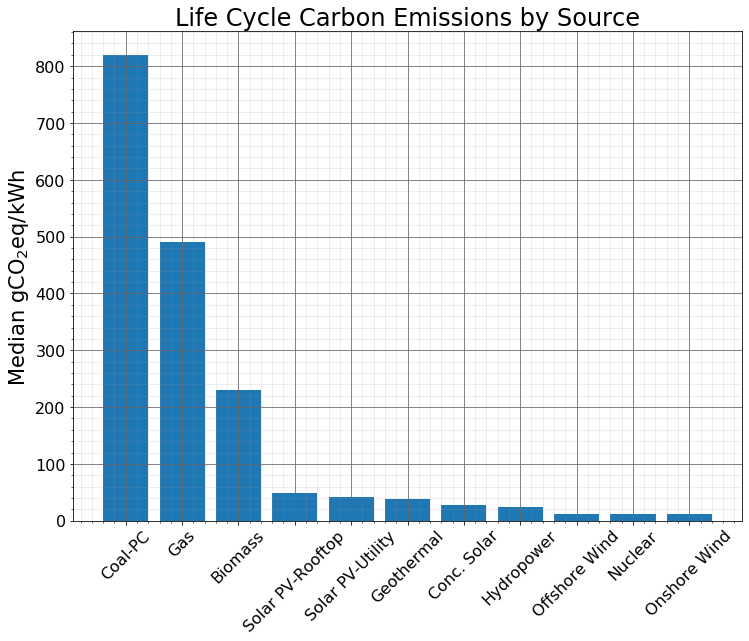
\includegraphics[width=\columnwidth]{co2emissions_source.png}
  \caption{The carbon lifecycle carbon emissions by energy source. Data is from
  IPCC 2018 Report on Climate Change \cite{allen_framing_2018}.}
  \label{fig:co2sources}
\end{figure}

 \glspl{esom} are useful for
exploring different policy scenarios and energy mixes when faced with future
uncertainty
\cite{decarolis_modelling_2016,hunter_modeling_2013,li_open_2020,decarolis_multi-stage_nodate}.
In this work, we use an \gls{esom} called \gls{temoa}
to analyze future energy mixes that will allow \gls{uiuc} to meet the
\gls{icap} goals \cite{decarolis_tools_2020}. This study is unique because we do
not consider all possible technologies that could replace natural gas and coal
capacity, which have a range of maturity and readiness. Rather, we
consider \gls{uiuc}'s existing energy mix and use \gls{temoa} to find the
minimum capacity of a nuclear power plant that will enable \gls{uiuc} to
satisfy its emissions goals.

We first examine a business-as-usual model to verify that \gls{temoa} agrees
with the findings in the Master Plan
\cite{affiliated_engineers_inc_utilities_2015}. Then we consider three scenarios
that introduce a nuclear power plant to the energy mix. Finally we employ an
uncertainty analysis method known as \gls{mga} to evaluate futures
that also meet the emissions limits for \gls{uiuc} but where system cost is not
perfectly minimized.
